%  .d8888b.        d8888 888888b.   8888888888
% d88P  Y88b      d88888 888  "88b  888
% 888    888     d88P888 888  .88P  888
% 888    888    d88P 888 8888888K.  8888888
% 888    888   d88P  888 888  "Y88b 888
% 888    888  d88P   888 888    888 888
% Y88b  d88P d8888888888 888   d88P 888
%  "Y8888P" d88P     888 8888888P"  8888888888
%
% Copyright (c) 2025, Abe Mishler
% Licensed under the Universal Permissive License v 1.0
% as shown at https://oss.oracle.com/licenses/upl/.
%
% A letter-size handout of the Big-O chart and
% common growth rates.
% 

\documentclass[10pt]{article}
\usepackage{geometry}
\geometry{papersize={8.5in,11in}, top=0.75in, bottom=0.75in, left=0.5in, right=1.25in} 

\usepackage{ragged2e}
\usepackage[export]{adjustbox}
\usepackage{graphics}
\usepackage{caption}
\usepackage[table]{xcolor}
\usepackage{siunitx}

\DeclareMathAlphabet{\mathcal}{OMS}{cmsy}{m}{n}
\SetMathAlphabet{\mathcal}{bold}{OMS}{cmsy}{b}{n}
\newcommand{\bigO}{\mathcal{O}}

\usepackage{fancyhdr}
\usepackage{lastpage}
\fancypagestyle{plain}{
	\fancyhf{} % clear all header and footer fields
	%\fancyfoot[L]{Rev.250310}
	\fancyfoot[C]{\hspace{1in}big$\bigO$chart.com}
	\renewcommand{\headrulewidth}{0pt}
	\renewcommand{\footrulewidth}{0pt}
}

\author{}
\title{\vspace{-2cm}} % Algorithm Analysis
\date{\vspace{-1.5cm}}
\pagenumbering{gobble}

\begin{document}
	
\maketitle

\begin{figure}[h!]
\begin{flushright}
	\begin{minipage}{6.5in}
		%\textbf{\Large Algorithm Analysis using $\bigO(g(n))$}\par\medskip
		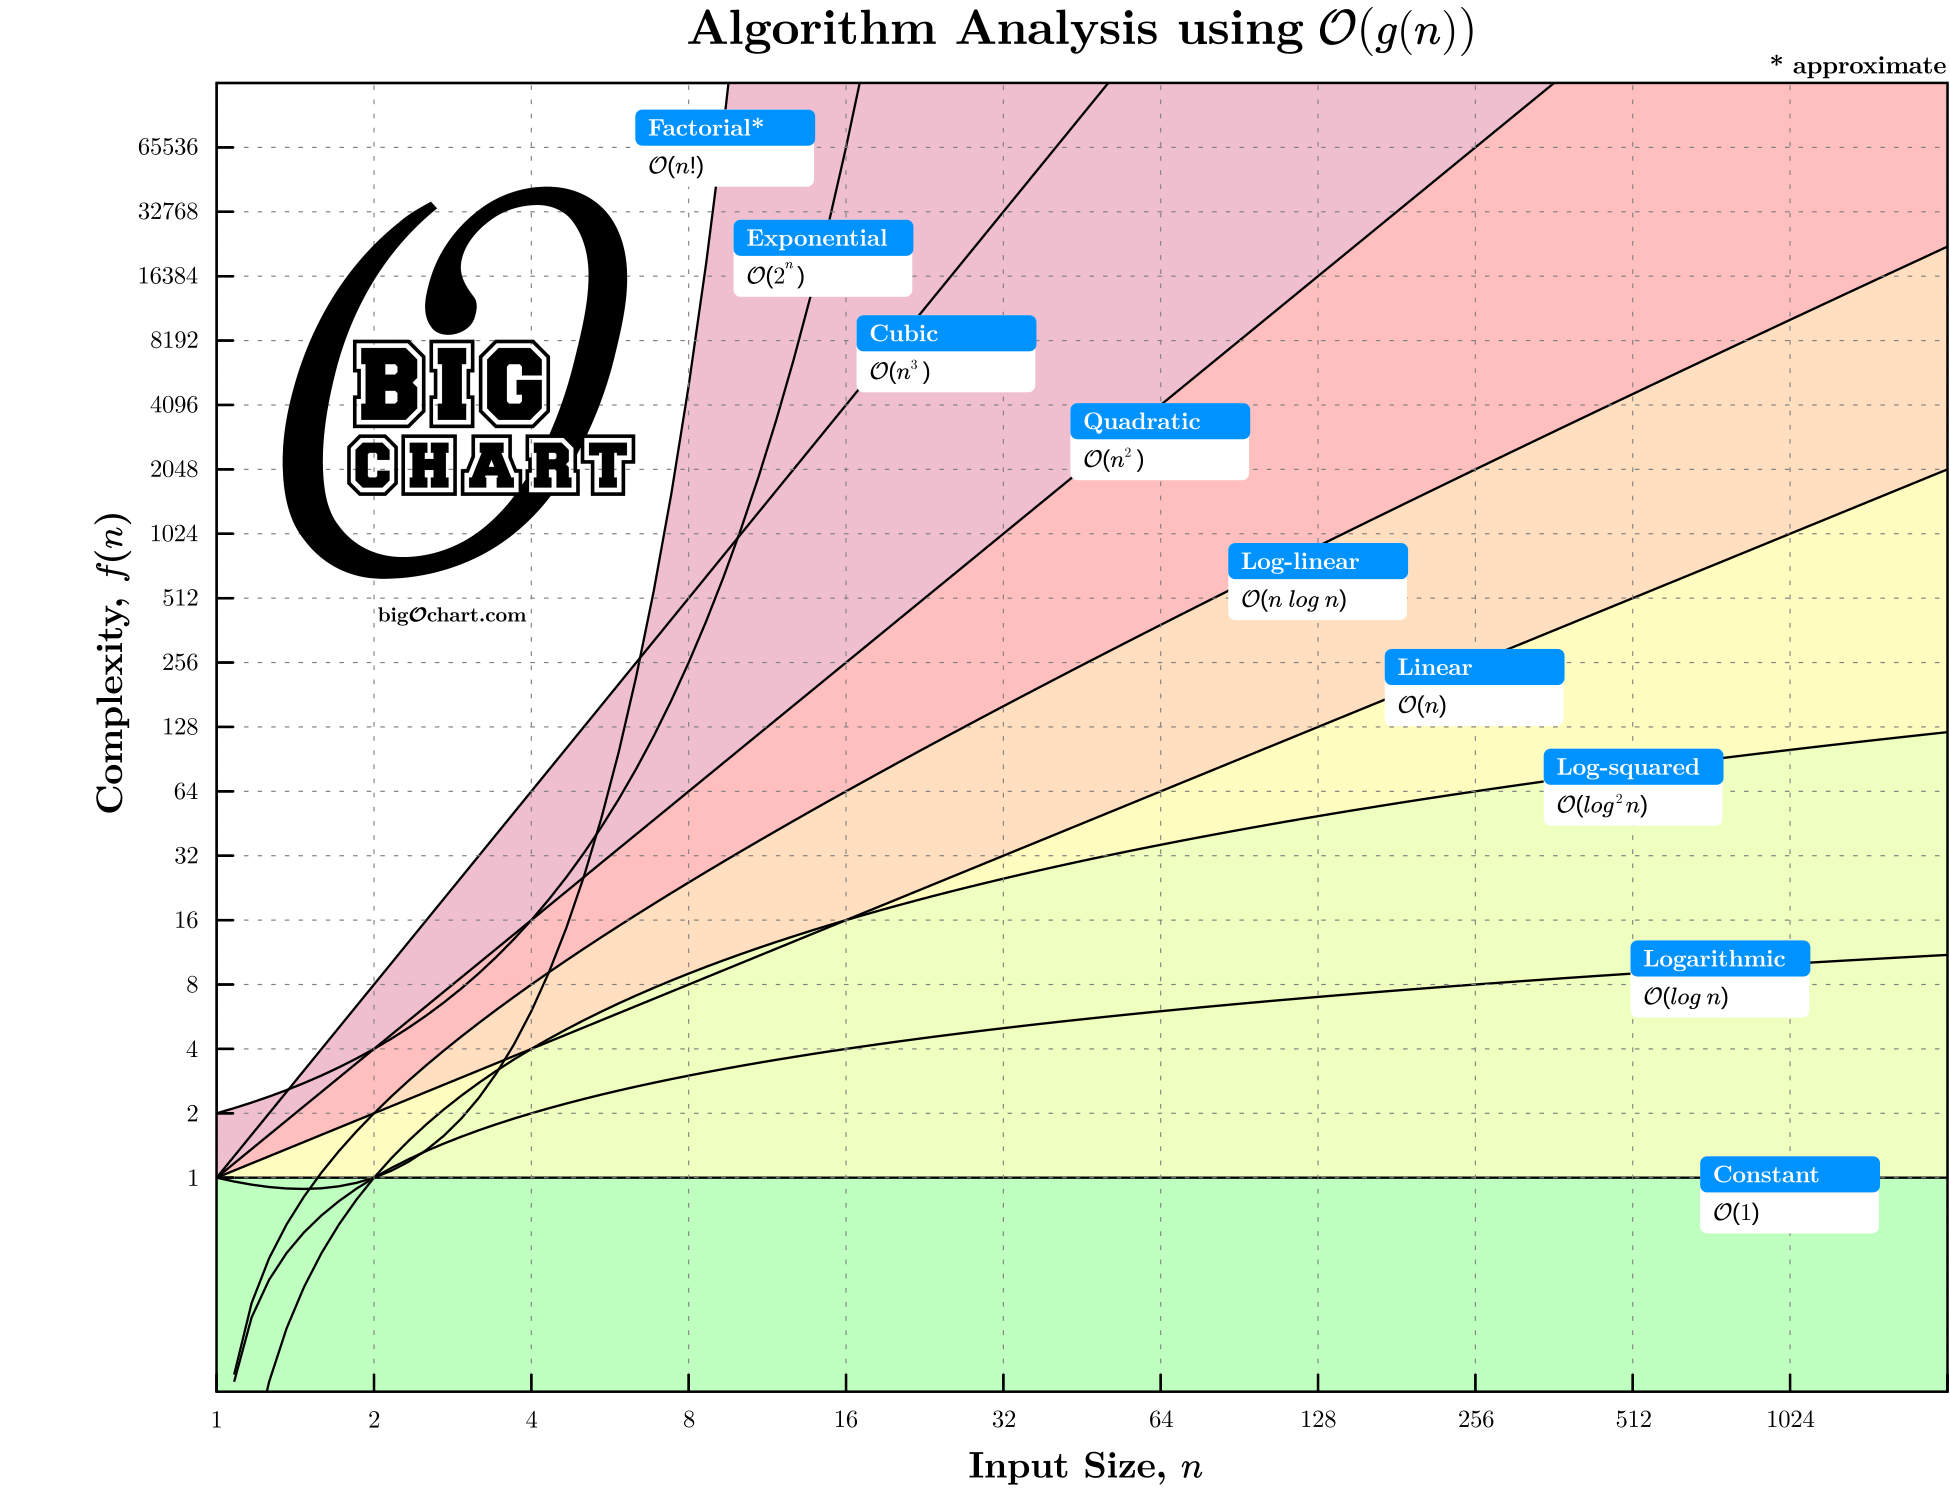
\includegraphics[width=468pt]{bigochart_6.5x5.png}
		\captionsetup{margin={2.5cm,0.75cm},justification=justified}
		\caption[]{$\bigO$-notation, a.k.a. "Big-O", is used to express the asymptotic upper bound on $f(n)$ by some constant multiple of $g(n)$, written as $f(n) = \bigO(g(n))$. This upper bound represents the growth of the worst case running time or space consumption and makes no claims regarding tightness of fit. The shaded area underneath each function depicts the absence of an asymptotic lower bound associated with $\bigO$-notation. See Table \ref{table:growthrates} for a partial numerical analysis.}
		\label{fig:bigochart}
	\end{minipage}
\end{flushright}
\end{figure}

\begin{table}[!h]
\begin{flushright}
	\begin{minipage}{6.5in}
		\begin{flushright}
			% resize the table, scale height proportionally
			% to 7in width (to fit on the page.)
			\resizebox{5.776in}{!}{
			\renewcommand{\arraystretch}{1.5}
			\begin{tabular}{|l|l|l|l|l|l|l|l|l|l|}
			\hline
			\bf{\textnumero} & \bf{Name} & \bf{$\bigO(g(n))$} & \multicolumn{7}{c|}{\bf{Complexity, $f(n)$}} \\
			\hline
			9 & \cellcolor{purple!25}Factorial & $\bigO(n!)$ & \num{2.09E+13} & \num{2.63E+35} & \num{1.27E+89} & \num{3.86E+215} &  &  & \\
			\hline
			8 & \cellcolor{purple!25}Exponential & $\bigO(2^n)$  & 65,536 & \num{4.29E+09} & \num{1.84E+19} & \num{3.40E+38} & \num{1.16E+77} & \num{1.34E+154} & \\
			\hline
			7 & \cellcolor{purple!25}Cubic & $\bigO(n^3)$ & 4,096 & 32,768 & 262,144 & 2,097,152 & \num{1.68E+07} & \num{1.34E+08} & \num{1.07E+09} \\
			\hline
			6 & \cellcolor{red!25}Quadratic & $\bigO(n^2)$ & 256 & 1,024 & 4,096 & 16,384 & 65,536 & 262,144 & 1,048,576 \\
			\hline
			5 & \cellcolor{orange!25}Log-linear & $\bigO(n\log n)$ & 64 & 160 & 384 & 896 & 2,048 & 4,608 & 10,240 \\
			\hline
			4 & \cellcolor{yellow!25}Linear & $\bigO(n)$ & 16 & 32 & 64 & 128 & 256 & 512 & 1,024 \\
			\hline
			3 & \cellcolor{lime!25}Log-squared & $\bigO(\log^2 n)$ & 16 & 25 & 36 & 49 & 64 & 81 & 100 \\
			\hline
			2 & \cellcolor{lime!25}Logarithmic & $\bigO(\log n)$ & 4 & 5 & 6 & 7 & 8 & 9 & 10 \\
			\hline
			1 & \cellcolor{green!25}Constant & $\bigO(1)$  & 1 & 1 & 1 & 1 & 1 & 1 & 1 \\
			\hline
			\multicolumn{3}{|r|}{\bf{Input Size, $n$}} & \bf{16} & \bf{32} & \bf{64} & \bf{128} & \bf{256} & \bf{512} & \bf{1,024} \\
			\hline
			\end{tabular}
			} % resizebox
		\end{flushright}
	\end{minipage}
\end{flushright}
\captionsetup{margin={-0.8cm,0cm},justification=justified}
\caption[]{Growth rates for algorithms with common complexities.}
\label{table:growthrates}
\end{table}
	
\end{document}
